\chapter{Servicios web}\label{chap:2}
\section{Instalación de infraestructura web}
Se ignora la primera parte de la sesión en esta práctica: la instalación local
de \Verb#nginx#. Se realizó sobre la marcha y no se refleja en la memoria ya que el
propio enunciado no lo considera relevante.

Respecto al resto del enunciado, se responden a las siguientes preguntas:
\begin{itemize}
	\item Tras la ejecución del primer comando, \Verb#netstat -4tpl# no muestra a
		nadie escuchando en el puerto 80 porque el contenedor Docker solo tiene
		SUS puertos abiertos, no los del anfitrión.
	\item Para ``averiguar'' la IP del contenedor, se ejecuta el siguiente comando: \\
		\begin{minipage}{\linewidth}
			\centering
			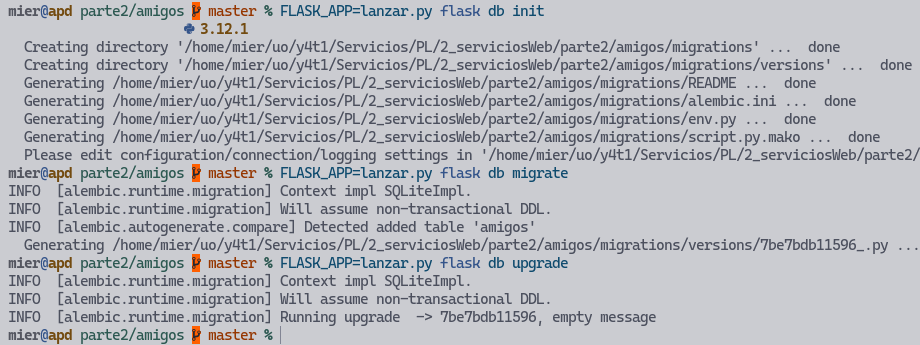
\includegraphics[width=\textwidth]{2/1.png}
			\captionof{figure}{Comando para obtener la dirección IP de un contenedor y resultado}\label{fig:2/1}
		\end{minipage}
	\item Al hacer \Verb#wget# a dicha IP se obtiene lo siguiente: \\
		\begin{minipage}{\linewidth}
			\centering
			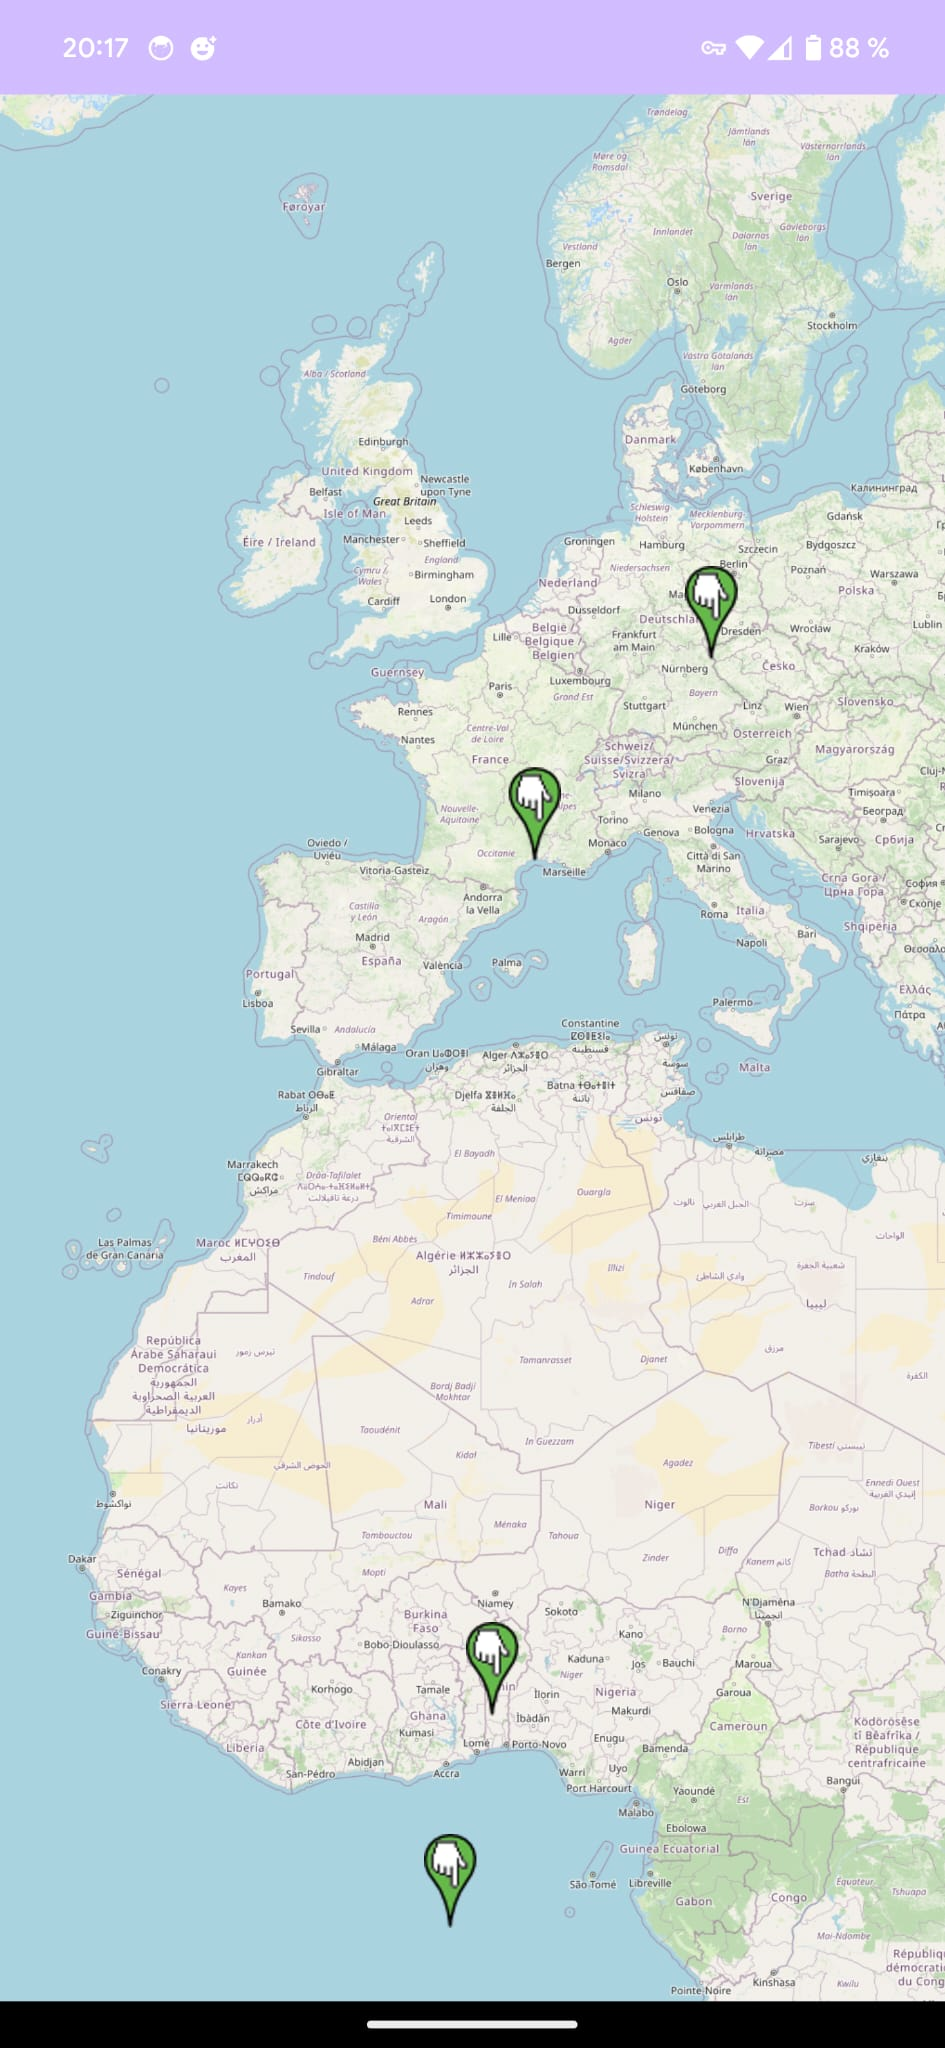
\includegraphics[width=\textwidth]{2/2.png}
			\captionof{figure}{Resultado de hacer wget a la IP del contenedor}\label{fig:2/2}
		\end{minipage}
	\item Se descarga el fichero \Verb#50x.html#: \\
		\begin{minipage}{\linewidth}
			\centering
			
\includegraphics[width=\textwidth]{2/3.png}
			\captionof{figure}{Descarga del fichero 50x.html}\label{fig:2/3}
		\end{minipage}
	\item Tras las modificaciones, se obtiene la siguiente respuesta (\textit{correcta}),
		y se comprueba que se ven las modificaciones en el navegador: \\
		\begin{minipage}{\linewidth}
			\centering
			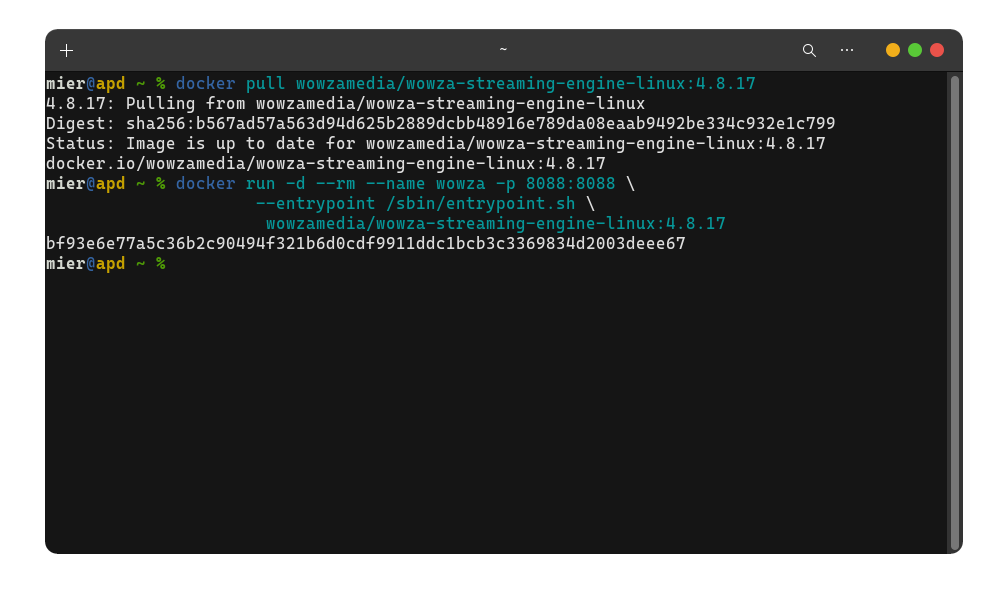
\includegraphics[width=\textwidth]{2/4.png}
			\captionof{figure}{Landing page de nginx}\label{fig:2/4}
		\end{minipage}
	\item En los logs del contenedor aparecen las peticiones del navegador: \\
		\begin{minipage}{\linewidth}
			\centering
			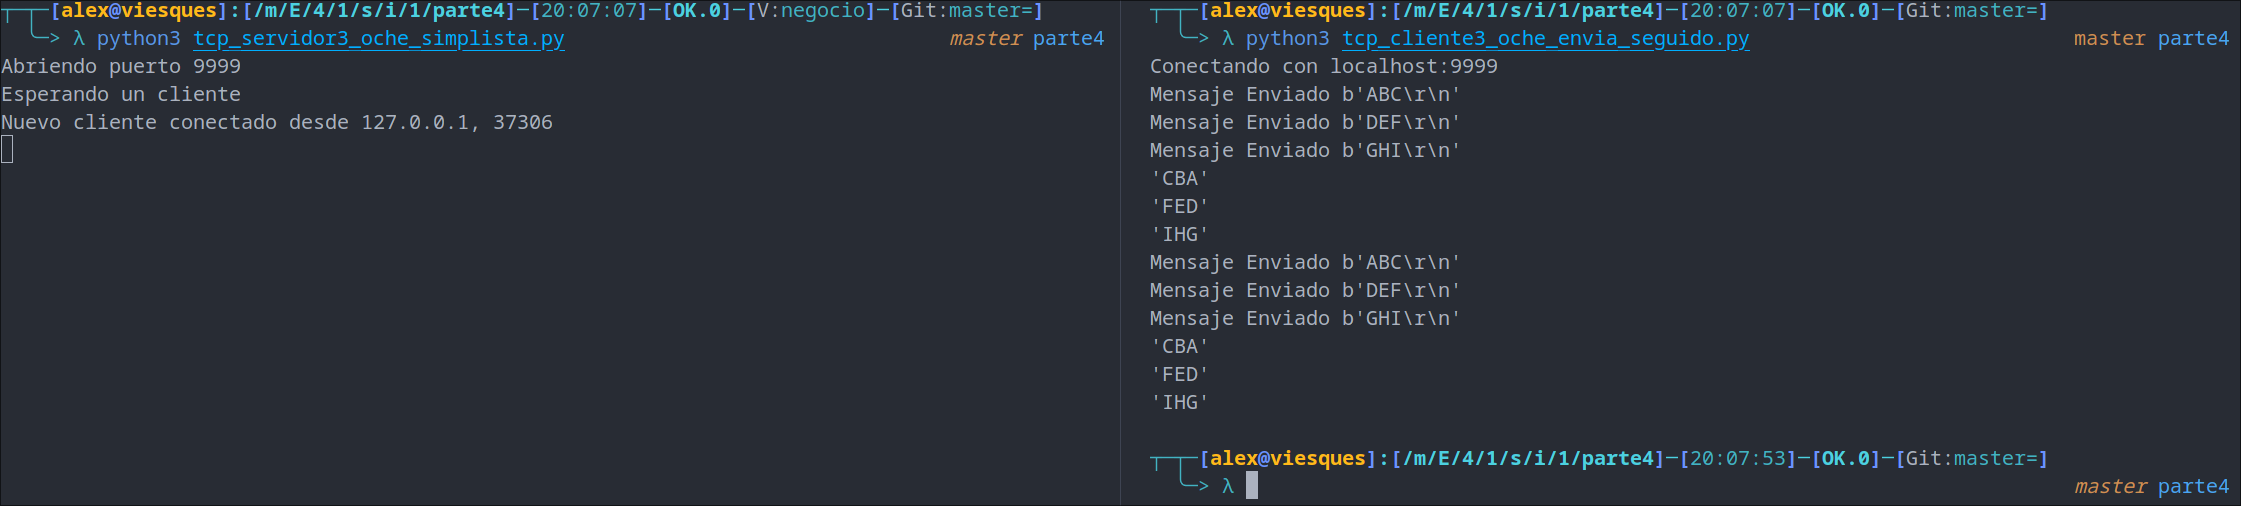
\includegraphics[width=\textwidth]{2/5.png}
			\captionof{figure}{Logs del contenedor}\label{fig:2/5}
		\end{minipage}
	\item Tras las modificaciones del enunciado, se prueba a acceder a un contenido
		que no existe: \\
		\begin{minipage}{\linewidth}
			\centering
			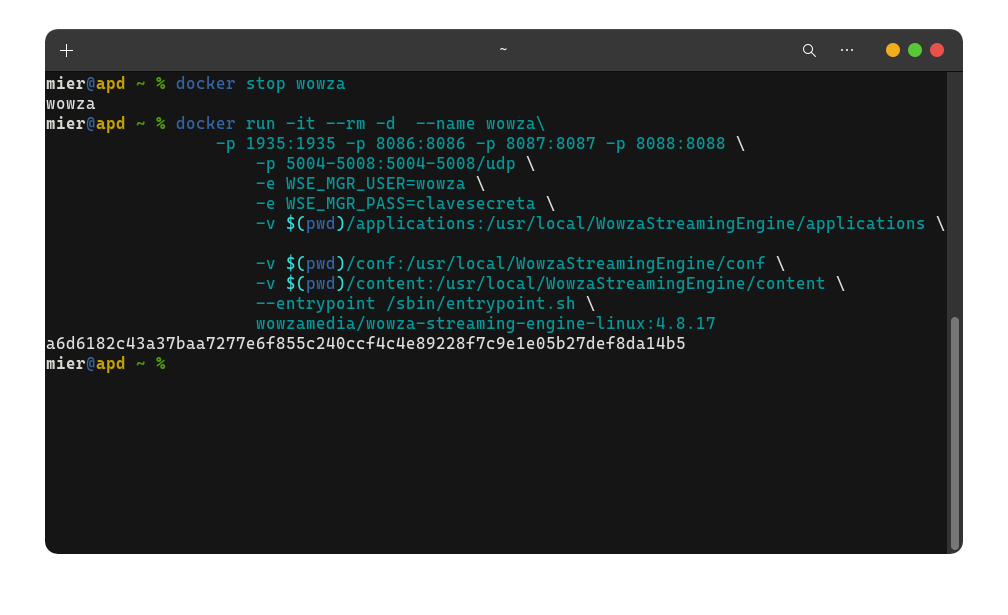
\includegraphics[width=\textwidth]{2/6.png}
			\captionof{figure}{404 al acceder a un contenido que no existe}\label{fig:2/6}
		\end{minipage}
\end{itemize}
\subsection{Ejercicio 1}
Se siguen todos los pasos y se comprueba que, al conectarse al otro puerto, se obtienen
respuestas distintas: \\
\begin{minipage}{\linewidth}
	\centering
	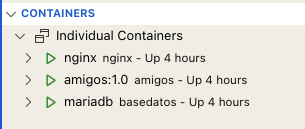
\includegraphics[width=\textwidth]{2/7.png}
	\captionof{figure}{Respuesta al acceder a otro puerto}\label{fig:2/7}
\end{minipage}

\subsection{Contenido dinámico (Flask)}
\textit{NOTA:~la práctica se realiza en un shell distinto de bash, por lo que se ejecutan
	los comandos de forma distinta a como se muestra en el enunciado para entrar en el
	entorno virtual.}

Se crea una carpeta separada con los ficheros relevantes: \\
\begin{minipage}{\linewidth}
	\centering
	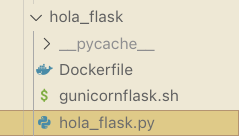
\includegraphics[width=\textwidth]{2/8.png}
	\captionof{figure}{Estructura de ficheros}\label{fig:2/8}
\end{minipage}

Se prueba la conexión de manera simple contra el servidor Flask: \\
\begin{minipage}{\linewidth}
	\centering
	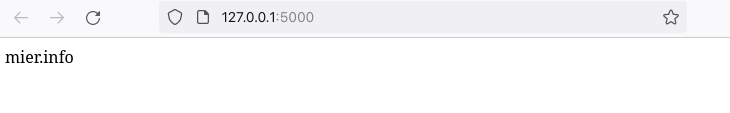
\includegraphics[width=\textwidth]{2/9.png}
	\captionof{figure}{Conexión a Flask}\label{fig:2/9}
\end{minipage}

Se realiza una conexión contra \Verb#gunicorn# y se comprueba que funciona: \\
\begin{minipage}{\linewidth}
	\centering
	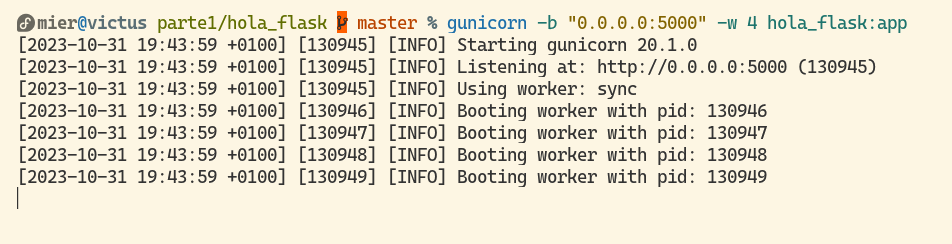
\includegraphics[width=\textwidth]{2/10.png}
	\captionof{figure}{Logs de gunicorn tras la prueba de conexión}\label{fig:2/10}
\end{minipage}
\\
\begin{minipage}{\linewidth}
	\centering
	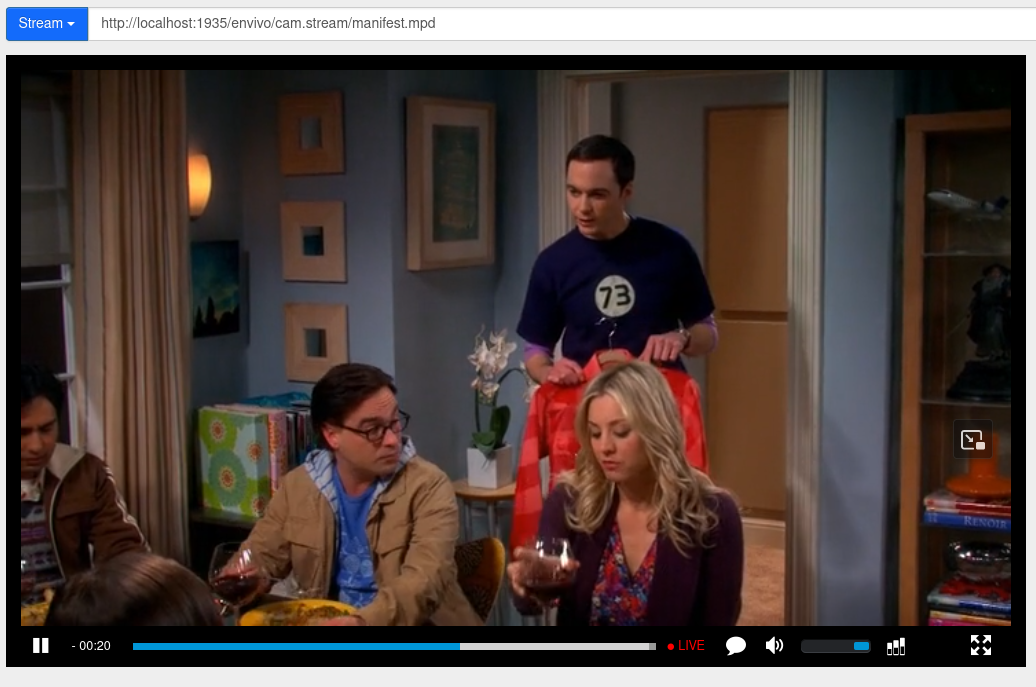
\includegraphics[width=\textwidth]{2/11.png}
	\captionof{figure}{Reflejo del navegador de la conexión con gunicorn}\label{fig:2/11}
\end{minipage}

\subsection{Ejercicio Dockerfile}
Se crea el fichero \Verb#Dockerfile# con el contenido del enunciado y se construye la
imagen: \\
\begin{minipage}{\linewidth}
	\centering
	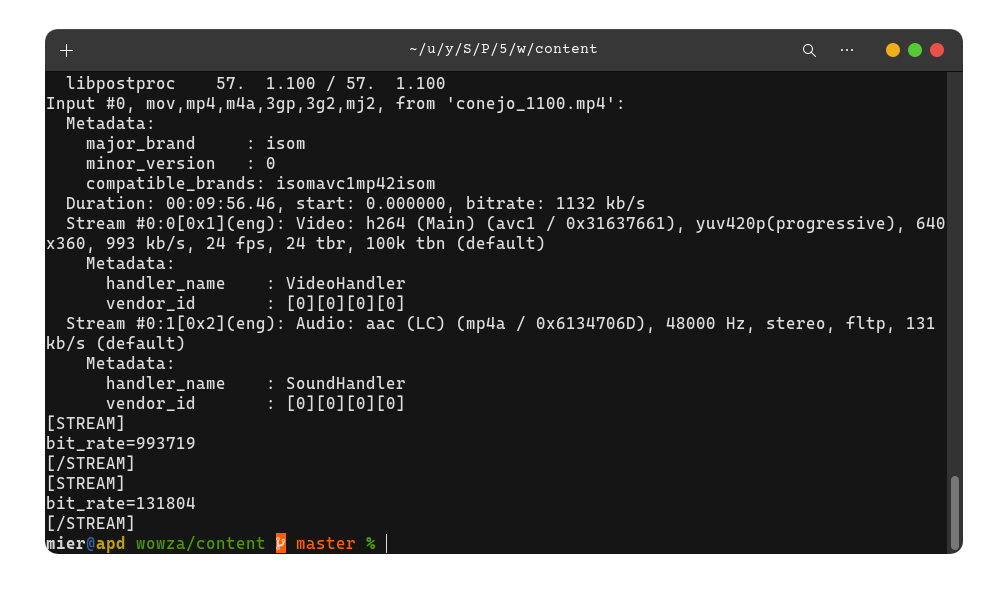
\includegraphics[width=\textwidth]{2/12.png}
	\captionof{figure}{Construcción y ejecución de la imagen}\label{fig:2/12}
\end{minipage}

Se comprueba que funciona correctamente: \\
\begin{minipage}{\linewidth}
	\centering
	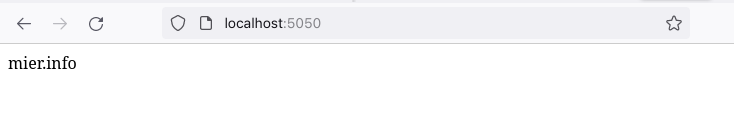
\includegraphics[width=\textwidth]{2/13.png}
	\captionof{figure}{Comprobación de conexión con la imagen}\label{fig:2/13}
\end{minipage}

\section{Aplicaciones web y HTTP}
